\section{Experiments \emph{\&} Results}
\label{sec:results}

We chose the MovieLens dataset\footnote{
See http://www.grouplens.org/node/73 --- accessed 10.05.2011}
to test the performance of our system.
This dataset is often used to test the performance of recommender systems
(as described in 
\cite[p9]{Alshamri2008}, \cite[p4]{Lemire2005}, \cite[p1]{Adomavicius2005} and \cite[p2]{Herlocker2004}).
It consists of a set of users, a set of movies, and a set of movie ratings from users,
on the scale $1$ through $5$.
We chose a subset of the entire MovieLens collection, with 100,000 ratings from 943 users on 1,682 movies.
The dataset was split into disjoint sets
($D = \{ d_1, ..., d_5 \}$) to perform five-fold cross-validation.

To evaluate how our model performs during prediction aggregation, 
we need a measure for computing the total error across a large number of predictions.
The canonical measure for estimating the error of a recommender system
is the \emph{Root mean squared error} (RMSE) measure
(for example in \cite[p17]{Herlocker2004}, \cite[p13]{Adomavicius2005} and \cite[p6]{Bell2007}).
We shall use this measure to estimate the performance
of our adaptive prediction aggregation algorithms.
The RMSE of a set of estimations $\hat{R}$, 
compared the correct rating values $R$, is defined as

\begin{equation*}
  \mathrm{RMSE}(\hat{R},R) = \sqrt{\mathrm{E}((\hat{R} - R)^2)}
  = \sqrt{\frac{
      \sum_{i=1}^{n} (\hat{R}_i - R_i)^2
    }{
      n
    }},
\end{equation*}

where $n$ is the total number of predictions.
The RMSE combines a set of errors into one single combined error.
A beneficial feature of the RMSE is that the resulting error 
will be on the same scale as the estimations. For example,
if we are predicting values on the scale $1-5$, the computed error
will be on this scale as well. In this case, an error of $1$
would then say that we are on average $1$ point away from the true 
ratings on our $1-5$ scale.

In addition to the dataset, we need a collection of recommender systems.
Standard recommenders will be used for both the basic predictions,
and the accuracy estimations,
as described in Section \ref{sec:adaptive}.

Naturally, we need a large number of different recommenders, preferably ones that consider
disjoint patterns in the data. Table \ref{table:results:methods}
gives a short overview of the recommender systems we shall employ.
Each experiment will use every recommender in this table.
This section only gives a short introduction to each recommender.

\subsection{Basic Recommenders}

\begin{table}
  \caption[Adaptive Modeling Methods]{
    adaptive modeling methods: A short overview of each of the recommender methods
    used in our experiment.
    Each recommender is used in every experiment. 
  }
  \setlength{\extrarowheight}{0.2em}
  \vspace{1em}
  \begin{tabular*}{0.48\textwidth}{ l l l l }
    \hline
    { } & \textbf{method} & \textbf{algorithm} & \textbf{description} \\
    \hline
    S & svd1          & SVD                   & ALSWR factorizer, 10 features. \\
    S & svd2          & SVD                   & ALSWR factorizer, 20 features. \\
    S & svd3          & SVD                   & EM factorizer, 10 features. \\
    S & svd4          & SVD                   & EM factorizer, 20 features. \\
    S & slope\_one    & Slope One             & Rating delta computations. \\
    S & item\_avg     & Baseline              & Item averages. \\ 
    S & baseline      & Baseline              & User and item averages.\\ 
    S & cosine   	    & Cosine sim.           & From similar items.\\ 
    S & knn       	  & Pearson Corr.         & From similar users.\\
    \hline
    A & median    	  & Aggregation           & Median aggregate rating. \\
    A & average    	  & Aggregation           & Average aggregate rating. \\
    A & adaptive      & Adaptive agg.         & Our approach. \\
    \hline
  \end{tabular*}
  \label{table:results:methods}
\end{table}

As seen in Table \ref{table:results:methods}, we have two types of recommenders:
First, we have the basic recommenders, denoted by \emph{S} in the table.
These recommenders each look at the data in different ways to arrive at predicted ratings.
We chose this wide range of recommenders for just this reason:
as previously explained, the performance of aggregate recommenders
are more dependent on the dissimilarity of the basic recommenders
than their individual performance.

Let us briefly explain how each basic recommender works.
In recommender systems, SVD is used to compress the ratings space into what is sometimes called a \emph{taste space},
where users are mapped to higher-level "taste" categories
(e.g. \cite[p5]{Ahn2004}, \cite[p4]{Brand2003} or \cite[p2]{Liu2006}).
The factorizers refers to algorithms used to factorize the ratings matrix
(e.g. the ALSWR factorizer \cite{Zhou2008}).

The Slope One and baseline algorithms look at average
ratings for items and from users, and use these to predict ratings.
These are simple algorithms that often perform as well
as more complex approaches.

The cosine similarity algorithm looks for items that are rated
similarly by the same users, and infers item similarity from this measure.
New ratings are then predicted by taking known ratings of other items,
weighted by their item's similarity to the new item.

The KNN algorithm employs yet another approach. This algorithm,
similar in strategy to the cosine similarity algorithm,
looks for users with similar rating patterns.
The similarity is measured with the Pearson Correlation Coefficient.
Predictions are created by collecting ratings from similar users
of the item in question, weighted by their respective similarity.
See \cite{Adomavicius2005}, \cite{Pazzani2007} or \cite{Schafer2007}
for a more comprehensive exploration of different types of recommenders.


\subsection{Aggregate Recommenders}

The second type of recommenders are the aggregation methods, 
that combine the result of each of the basic recommender systems
(the methods below the middle line in Table \ref{table:results:methods},
denoted "A").
The first two of these methods are simple aggregation approaches.
The median aggregation method choses the median value of the predictions
produced by the standard recommenders.
Similarly, the average aggregation method takes the mean of the
standard predictions.
While not complex in nature, these methods
will help us see how our method compares to simple, traditional
aggregation techniques.

The last entry in Table \ref{table:results:methods}
refers to our technique. 
This is the recommender outlined by Section \ref{sec:adaptive},
that create secondary accuracy estimating recommender systems,
in order to adaptively weigh each basic recommender.
All the aggregation approaches, including our technique,
use every basic recommender system described so far.

As explained in Section \ref{sec:adaptive},
any basic recommender system can be used for the adaptive method.
The only difference is how this method is trained:
while the basic methods are trained using the ratings matrix,
the adaptive methods are trained using the error model.
In other words, we have as many possibilities for choosing
the adaptive recommenders as the basic recommenders.

For our experiment, we went with SVD recommenders
for each of the adaptive models.
That is, each basic recommender method gets a secondary 
accuracy predicting recommender, which in this case is a 
standard SVD recommender.
The SVD recommender is a natural choice in this case,
since we wish to uncover latent patterns of accuracy
for each model.
Examples of these patterns include groups of items
or users a specific recommender works well for.

It is important to note that the same configuration of recommenders was used for all three experiments.
In other words, neither the basic nor the aggregate or adaptive recommenders were heavily tailored
to each dataset. To be sure, higher performance could probably have been achieved
by tailoring each recommender to each dataset. However,
as our goal is to compare our finite set of methods, all we care 
about is how they perform compared to each other.

As with the basic recommenders, the same SVD recommender configuration was used 
for the adaptive layer in each Experiment.
We chose to use en EM-factorizer to perform the actual decomposition,
consisting of 20 features. The decomposition was performed by 20 iterations.


\subsection{Results}

Table \ref{table:results:e1} gives the resulting RMSE values when our algorithm is used with the MovieLens dataset.
Each cell corresponds to the RMSE values for each dataset,
for each recommender and aggregation approach.
The bottom entry in this table refers to our adaptive recommenders method.
As seen in this table, our approach outperforms both the standard recommenders
and the aggregation approaches.

By outperform we mean that our model should have a lower
mean RMSE score than the other singular methods. As we can see in Table \ref{table:results:e1},
our approach outperforms both the standard recommenders
and simple generalized aggregation approaches.
While we can not generalize too much on this basis, 
the fact that this dataset is a common testing ground for recommender systems,
and that RMSE is the de facto measure for determining performance,
we have grounds for some confidence in these results.

\begin{table}
  
  \centering
  \tiny
  (a) RMSE values for the five disjoint subsets:

  \vspace{0.4em}

  \begin{tabular*}{0.9\textwidth}{ l l l l l l l }
    \hline
    { } & method & $d_1$ & $d_2$ & $d_3$ & $d_4$ & $d_5$ \\ 
    \hline
    S & svd1          & 1.2389	  & 1.1260	  & 1.1327	  & 1.1045	  & 1.1184	 \\
    S & svd2          & 1.2630	  & 1.1416    & 1.1260	  & 1.1458	  & 1.1260	 \\
    S & svd3          & 1.0061	  & 0.9825	  & 0.9830	  & 0.9815	  & 0.9797	 \\
    S & svd4          & 1.0040	  & 0.9830	  & 0.9849	  & 0.9850	  & 0.9798	 \\
    S & slope\_one    & 1.1919	  & 1.0540	  & 1.0476	  & 1.0454	  & 1.0393   \\
    S & item\_avg     & 1.0713	  & 0.9692	  & 0.9662	  & 0.9683	  & 0.9725	 \\
    S & baseline       & 1.0698	  & 0.9557	  & 0.9527	  & 0.9415	  & 0.9492	 \\
    S & cosine   	    & 1.1101	  & 0.9463	  & 0.9412	  & 0.9413	  & 0.9382	 \\
    S & knn       	  & 1.4850	  & 1.1435	  & 1.1872    & 1.2156	  & 1.2022	 \\
    \hline                                                                    
    A & median    	  & 0.9869	  & 0.8886	  & 0.8857    & 0.8857	  & 0.8855	 \\
    A & average    	  & 0.9900	  & 0.8536	  & 0.8525	  & 0.8525	  & 0.8519	 \\
    A & adaptive       & \textbf{0.9324}	  & \textbf{0.8015}	  & \textbf{0.7993}  & \textbf{0.8238} & \textbf{0.8192} \\
    \hline
  \end{tabular*}

  \vspace{1em}
  
  (b) Statistics for the methods:

  \vspace{0.4em}

  \begin{tabular*}{0.9\textwidth}{ l p{1.8cm} l l l l l }
    \hline
    { } & method & min & max & mean & $\sigma$ & $\Delta$ \\
    \hline
    S & knn       	  & 1.1435	& 1.4850	& 1.2467	& 0.3487 & - \\
    S & svd2          & 1.1260	& 1.2630	& 1.1605	& 0.2277 & 6.9\% \\
    S & svd1          & 1.1045	& 1.2389	& 1.1441	& 0.2197 & 1.4\% \\
    S & slope\_one    & 1.0393	& 1.1919	& 1.0756	& 0.2415 & 5.9\% \\
    S & item\_avg     & 0.9662	& 1.0713	& 0.9895	& 0.2023 & 8.0\% \\
    S & svd4          & 0.9798	& 1.0040	& 0.9873	& \textbf{0.0924} & 2.2\% \\
    S & svd3          & 0.9797	& 1.0061	& 0.9865	& 0.0991 & 0.1\% \\
    S & cosine   	    & 0.9382	& 1.1101	& 0.9754	& 0.2595 & 1.1\% \\
    S & baseline       & 0.9415	& 1.0698	& 0.9738	& 0.2196 & 1.6\% \\
    \hline            
    A & median    	  & 0.8855	& 0.9865	& 0.9065	& 0.2005 & 6.9\% \\
    A & average    	  & 0.8519	& 0.9900	& 0.8801	& 0.2344 & 2.9\% \\
    A & adaptive       & \textbf{0.7993}	& \textbf{0.9324}	& \textbf{0.8352}	& 0.2225 & 5.1\% \\
    \hline
  \end{tabular*}
  \label{table:results:e1}
\end{table}

Statistics for each experiment are given in the last
part of Table \ref{table:results:e1}. 
The statistical values are the minimum, maximum and mean values
for each of the methods. We also include
the standard deviation ($\sigma$) for each method,
across each collection of subsets.
This table confirms the results from the full results table:
Our adaptive recommenders approach improves the mean performance
of our system.
The mean performance and the standard deviation
are shown in Figure \ref{plot:movielens}.

\begin{figure}[t]
\center

\pgfplotsset{width=\textwidth,height=8cm}
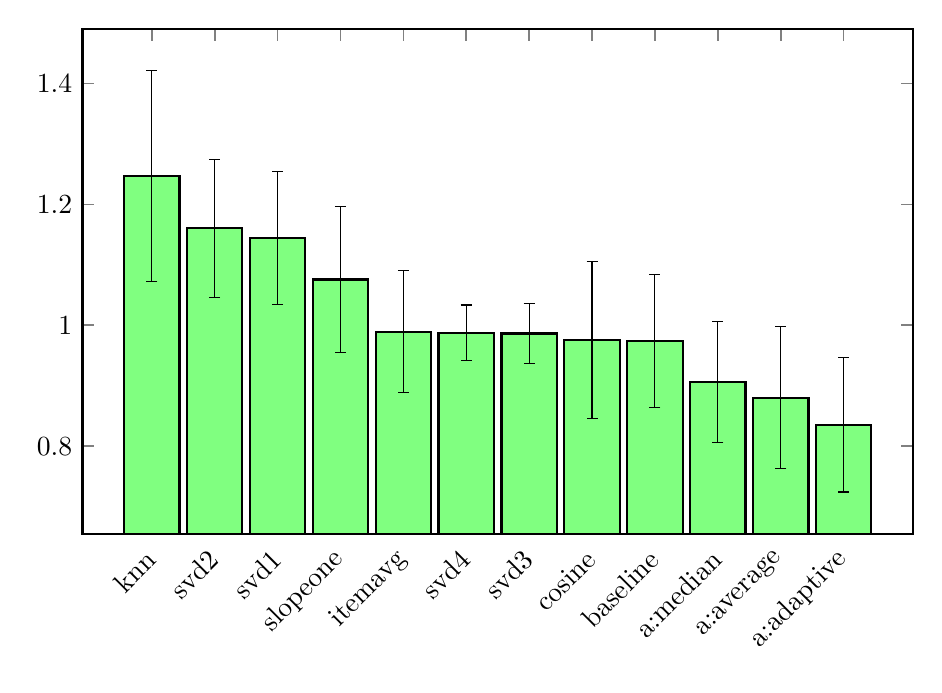
\begin{tikzpicture}

\begin{axis}[
      symbolic x coords={
        knn,svd2,svd1,slopeone,itemavg,svd4,svd3,cosine,baseline,a:median,a:average,a:adaptive},
      xtick=data,
      x tick label style={rotate=45,anchor=east,yshift=-0.5em,xshift=-0.2em},
      bar width=20pt
    ]

    \addplot [ybar,fill=green!50,error bars/.cd,y dir=both,y explicit] coordinates {
      (knn, 1.2467) +- (0,0.17435) 
      (svd2, 1.1605) +- (0,0.11385)
      (svd1, 1.1441) +- (0,0.10985)
      (slopeone, 1.0756) +- (0,0.12075)
      (itemavg, 0.9895) +- (0,0.10115)
      (svd4, 0.9873) +- (0,0.0462)
      (svd3, 0.9865) +- (0,0.04955)
      (cosine, 0.9754) +- (0,0.12975)
      (baseline, 0.9738) +- (0,0.1098)
    %};
    %\addplot [ybar,fill=blue!50] coordinates {
      (a:median, 0.9065) +- (0,0.10025)
      (a:average, 0.8801) +- (0,0.1172)
      (a:adaptive, 0.8352) +- (0,0.11125)
    };
\end{axis}

\end{tikzpicture}
\caption[Average RMSE Plot]{
  Average RMSE plot: This plot shows the average RMSE for each method, and each aggregation method (denoted "a:").
  The actual numbers are given in Table \ref{table:results:e1}.
  The error bars indicate the standard deviation of each method.
  Note the scale on the y-axis --- the errors are not as pronounced as they might seem. 
  See also Figure \ref{plot:datasets}.
}
\label{plot:rmse}
\end{figure}




%\begin{figure}
\center

\pgfplotsset{width=\textwidth,height=8cm}
\pgfplotsset{every axis/.append style={
thick,
tick style={semithick}}}

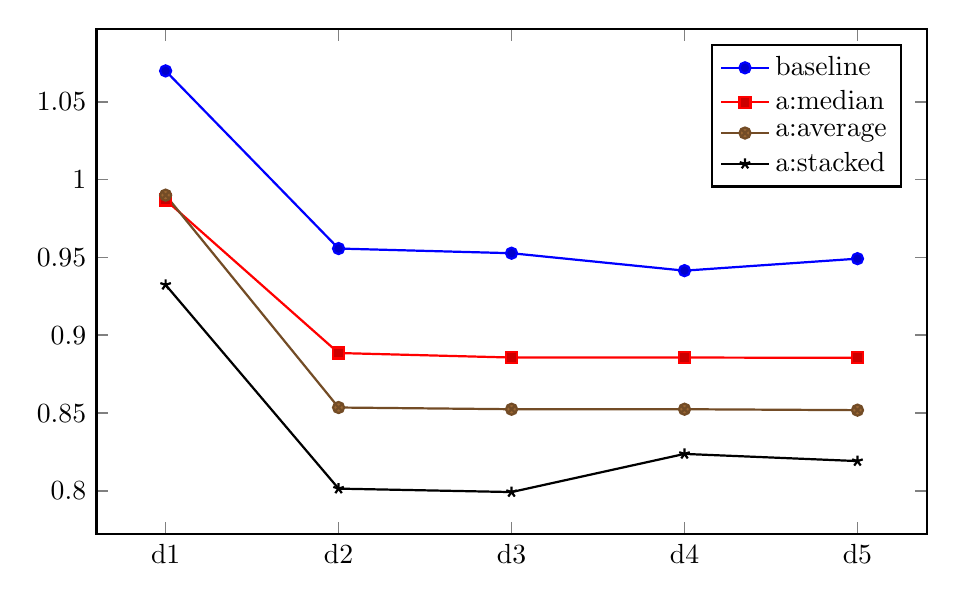
\begin{tikzpicture}

\begin{axis}[
  stack plots=false,
  enlarge x limits=true,
  symbolic x coords={d1,d2,d3,d4,d5},
  xtick=data,
  legend style={
    cells={anchor=west},
    legend pos=north east,
  }
]

\addplot coordinates {
(d1, 1.0698)
(d2, 0.9557)
(d3, 0.9527)
(d4, 0.9415)
(d5, 0.9492)
};
\addlegendentry{baseline}


\addplot coordinates {
(d1, 0.9869)
(d2, 0.8886)
(d3, 0.8857)
(d4, 0.8857)
(d5, 0.8855)
};
\addlegendentry{a:median}
 
\addplot coordinates {
(d1, 0.9900)
(d2, 0.8536)
(d3, 0.8525)
(d4, 0.8525)
(d5, 0.8519)
};
\addlegendentry{a:average}
 
\addplot coordinates {
(d1, 0.9324)
(d2, 0.8015)
(d3, 0.7993)
(d4, 0.8238)
(d5, 0.8192)
};
\addlegendentry{a:stacked}

\end{axis}
\end{tikzpicture}

\caption[RMSE Variations]{
  RMSE Variations: This plot shows that, while the standard deviation of each method may be high,
  this has more to do with the selected dataset than with their performance in comparison with each other.
  The performance of each of the aggregate methods, as well as the baseline standard method,
  follow similar performance paths across the disjoint datasets.
}
\label{plot:datasets}
\end{figure}






Let us take a look at the standard deviation measures from the different methods.
As seen in Figure \ref{plot:movielens}, 
most of the methods, including the adaptive models,
exhibit quite a lot of variation in their results.
If these variations occurred as a result of unstable
predictions of the same dataset, this would be a substantial problem,
resulting in unreliable predictions.
However, the standard deviation is mostly caused by the differing
performance across the varying datasets.
As we see, the performance of each of the aggregation methods,
as well as the best performing standard recommender,
follow each other closely. At the same time,
performance varies across the different datasets,
which results in high values for $\sigma$.

There are two important limitations.
First, our approach is much more complex than those we test it against.
The question whether the methods performance is worth its extra complexity becomes important.
Second, the generalized aggregation methods we chose to test our method with
are simpler than the most powerful modern approaches to aggregate recommenders.
This fundamentally limits how confident we can be that our system
is indeed an improvement.
We shall discuss this further in Section \ref{sec:discussion}.

\cite{Bjorkoy2011} performs more experiments with adaptive recommenders,
including one where this approach is used to provide personalized search results.


